% =====================================================================
%  AI-ASSISTED DRAFT. The prose was AI-drafted from the author's results; the
%  research design, decisions, and interpretation are the author's own, and AI
%  assistance is disclosed in the Acknowledgments. Every number traces to
%  results/*.csv (via analyze.py / analyze_kill.py). Figures are AI-generated
%  and marked. Swap this preamble for a venue style file at submission.
% =====================================================================
\documentclass[11pt]{article}
\usepackage[margin=1in]{geometry}
\usepackage{lmodern}
\usepackage[T1]{fontenc}
\usepackage{graphicx,booktabs,amsmath,amssymb,microtype,xcolor}
\usepackage[numbers,square]{natbib}
\usepackage{caption}
\captionsetup{font=small,labelfont=bf}
\graphicspath{{../results/figs/}}

\title{\textbf{Measuring What You Cannot See:\\ A Calibrated Study of Welfare and Equity Erosion\\ in Proxy-Optimizing Incentive Allocation}}
\author{[Author name and affiliation]}
\date{}

\begin{document}
\maketitle

\begin{abstract}
Organizations increasingly delegate resource-allocation decisions to systems that
optimize what they can measure. When the measurable target (employee retention)
is only a proxy for the true objective (employee welfare), optimization pressure
can silently erode the objective it cannot see. We study this in an open,
CPU-only agent-based testbed in which a budget-limited learner allocates five
incentive types across a heterogeneous workforce, observing retention but not a
latent satisfaction variable, with a tunable ``handcuff'' channel through which
monetary incentives raise retention \emph{without} raising satisfaction. Across
$200$ seeds we find that the retention-optimizing learner matches a theory-based
static allocator on observed retention while degrading latent satisfaction
($-0.037$ on a $[0,1]$ scale, $100\%$ seed-sign-stable) and roughly tripling
cross-archetype inequality. Through pre-registered falsification tests we show
this degradation is \textbf{not} an artifact of our assumptions: it persists at
zero crowding-out, on a never-left ``founder'' cohort (ruling out survivorship
composition), in $100\%$ of $250$ randomized parameter worlds, and---critically
---when the attrition hazard and archetype mix are \textbf{calibrated to the IBM
HR Analytics benchmark}, in which the off-satisfaction ``handcuff'' retention
channel is itself empirically present (stock-option coefficient $-0.51$
controlling for satisfaction). We frame this as a \emph{distributional}
sharpening of multitask principal--agent theory: a retention-optimizer does not
merely lower average welfare, it concentrates the loss on specific archetypes,
robustly and under calibration. We also test the natural remedy---a sparse audit
of the hidden objective folded into the reward---and report an honest
\emph{negative} result: the naive-estimator backfire we first observed appears
only under strong satisfaction--retention coupling; a precision-aware estimator,
\emph{or} the weaker coupling the benchmark actually exhibits, removes it. Audit
remedies matter only in a narrow regime. All code, data, the IBM calibration,
and a prompt log for AI-assisted implementation are released.
\end{abstract}

% =====================================================================
\section{Introduction}
Learning systems that allocate limited resources---advertising budget, clinical
attention, promotions, retention incentives---are typically rewarded on a
metric that can be logged. In personnel settings that metric is almost always
\emph{retention}: it is cheap to observe and directly tied to cost. The
construct the organization actually cares about---employee welfare, or
satisfaction---is expensive to observe and is measured, if at all, through
infrequent surveys. This gap between a cheap observable proxy and an expensive
latent objective is the classic precondition for Goodhart's law
\citep{strathern1997}: ``when a measure becomes a target, it ceases to be a
good measure.'' A large literature establishes that optimizing a proxy can
degrade the true objective, in economics \citep{holmstrom1991,baker1992} and in
machine learning \citep{amodei2016,krakovna2020,skalse2022,karwowski2024}. What
is far less understood is a practical, deployment-relevant question: if an
organization knows its allocator optimizes a proxy and can afford to
occasionally \emph{audit} the true objective, does that audit repair the damage?
And does the answer depend on how often it audits, or on how it uses what it
learns?

We study three research questions in a controlled simulation:
\begin{itemize}
  \item \textbf{RQ1 (Existence \& robustness).} Does optimizing an observable
  retention proxy degrade unobserved satisfaction and its distribution across
  worker types, and is that degradation robust to modelling choices rather than
  an artifact of a single hand-set parameter?
  \item \textbf{RQ2 (Harm vs.\ trapping).} If satisfaction falls, is it because
  workers are made less satisfied (per-person harm) or because unhappy workers
  who would have quit are retained (survivorship composition)?
  \item \textbf{RQ3 (Audit remedy).} Does auditing the hidden objective and
  folding it into the reward repair the degradation---and is the answer governed
  by audit \emph{frequency} or by how the audit signal is \emph{estimated}?
\end{itemize}

\noindent\textbf{Contributions.}
\begin{enumerate}
  \item \textbf{An open, reproducible testbed} for proxy-driven incentive
  allocation with a latent welfare variable, heterogeneous worker archetypes,
  intrinsic-motivation crowding-out, and a tunable unmediated-retention
  ``handcuff'' channel---CPU-only, standard-library, deterministic per seed.
  \item \textbf{Robust, calibrated evidence of \emph{distributional} welfare
  erosion.} A retention-optimizing learner degrades latent satisfaction and,
  more sharply, cross-archetype \emph{equity} (roughly $4\times$ the inequality of
  a static theory baseline) while matching that baseline on observed retention.
  We show (via a zero-crowding control, a founder-cohort metric,
  replacement-scheme sensitivity, a $250$-world randomized sweep, \emph{and}
  calibration of the hazard slope and archetype mix to the IBM HR Analytics
  benchmark) that the effect is not an assumption artifact. We frame it as a
  distributional sharpening of multitask agency \citep{holmstrom1991}: the loss
  concentrates on specific worker types, and the ``handcuff'' channel is
  empirically present in the benchmark (stock options).
  \item \textbf{An honest negative result on the audit remedy}, from two
  pre-registered falsification tests. A naive audit-reward estimator appears to
  backfire at low audit volume, but this vanishes both under a precision-aware
  estimator and under the weaker satisfaction--retention coupling the benchmark
  actually exhibits---so measurement helps at most in a narrow regime. We report
  in full the finding that \emph{failed} its kill-tests, not only the ones that
  survived.
  \item \textbf{Honest scope.} The study is a conditional, hypothesis-generating
  simulation with unitless parameters; we report where each finding is and is
  not robust, and outline a remote-only path to empirical calibration.
\end{enumerate}

% =====================================================================
\section{Related Work}
\textbf{Proxy optimization and reward hacking.} That optimizing an imperfect
proxy degrades the true objective is formalized for reinforcement learning by
Karwowski et al.~\citep{karwowski2024} and quantified as reward-model
overoptimization by Gao et al.~\citep{gao2023}; both study optimization
\emph{pressure} on generic objectives.
Conceptual treatments of specification gaming \citep{amodei2016,krakovna2020}
and a formal characterization of reward hacking \citep{skalse2022} establish the
phenomenon. Our contribution is orthogonal: we hold the optimizer fixed and ask
whether \emph{measuring} the hidden objective at a chosen frequency and
precision repairs the damage.

\textbf{Personnel economics.} The multitask principal--agent model
\citep{holmstrom1991} shows that strengthening incentives on a measurable task
diverts effort from an unmeasurable one; Baker~\citep{baker1992} shows that adding a
noisy measure of the true objective can \emph{reduce} welfare. Our RQ1 result is
a computational, heterogeneous-agent instantiation of these theorems---we
concede it is not a new mechanism---while our RQ3 audit result speaks directly to
Baker's noisy-measure concern with a concrete estimator-design remedy. The
behavioral anchors for our response model are intrinsic-motivation crowding-out
\citep{deci1999,frey2001} and the hygiene/motivator distinction
\citep{herzberg1959}; we use these for the \emph{sign and functional form} of
mechanisms only, not for calibrated magnitudes.

\textbf{Monitoring backfires.} Non-monotone effects of monitoring on human
effort are documented behaviorally via distrust and crowding-out
\citep{falk2006,dickinson2008}. Our audit backfire, when it appears, arises from
a different source---estimator variance in the learner, not worker
psychology---and, crucially, we show it is removable by estimator design, which
the behavioral backfires are not.

\textbf{RL for retention.} Prior applied work uses RL to \emph{maximize}
observed retention or customer value \citep{cheng2020}; none, to our knowledge,
characterizes the damage to an unobserved welfare construct or the estimator
dependence of an audit remedy.

% =====================================================================
\section{Model and Method}\label{sec:method}
\textbf{Workforce.} We simulate $N{=}400$ employees over $T{=}12$ quarters. Each
employee has one of four archetypes in equal share---low-compensation,
low-career-velocity, burnout-prone, and ambition-driven---whose structure and
archetype-to-incentive affinities extend a prior incentive taxonomy the author
derived from a public HR-analytics dataset. Each employee carries a latent
satisfaction $s\in[0,1]$; \emph{$s$ is a unitless illustrative variable and all
magnitudes below are non-calibrated modelling choices.}

\textbf{Incentives and dynamics.} Each quarter the allocator gives each employee
one of five incentive categories (monetary, recognition, flexibility,
development, social) or none, subject to a per-capita budget. An incentive
matched to an archetype's affinity raises $s$ with diminishing returns;
untreated $s$ drifts down; repeated identical incentives habituate. Monetary
incentives additionally impose a one-quarter-lagged crowding-out penalty on the
ambition and burnout archetypes \citep{deci1999,frey2001}.

\textbf{Attrition and the handcuff channel.} An employee leaves with probability
\begin{equation}
  \Pr(\text{leave}) = \sigma\!\left(\beta_0 - \beta_s\, s
    - h\,\mathbb{1}[\text{monetary in last two quarters}]\right),
  \label{eq:hazard}
\end{equation}
where $\sigma$ is the logistic function, $\beta_0$ and $\beta_s$ are illustrative
constants, and $h\ge 0$ is the \emph{handcuff strength}: the degree to which
recent monetary incentives suppress attrition \emph{without} raising
satisfaction (modelling vesting, switching costs, or non-competes). $h$ is the
wedge that decouples the observed proxy from the latent objective; we sweep it.
Leavers are replaced by fresh employees (sensitivity to this choice is tested in
\S\ref{sec:results}).

\textbf{Policies.} We compare six allocators: \emph{Random}; \emph{Monetary-only};
\emph{Static}, a theory-based rule assigning each archetype its affinity-matched
category (the strongest non-learning baseline); \emph{Learner}, a per-archetype
$\varepsilon$-greedy bandit rewarded on retention; \emph{Learner+audit}, which
additionally surveys a random fraction $p$ of employees each quarter and folds
the audited satisfaction into its reward; and \emph{Oracle}, which sees true $s$
(an upper bound). The learner maintains two per-cell estimates and selects the
action maximizing
\begin{equation}
  v(k,a) = \hat Q^{\text{stay}}(k,a) + \lambda\,\phi\!\big(\hat Q^{\text{sat}}(k,a), n_{k,a}\big),
  \label{eq:value}
\end{equation}
where $k$ is the archetype, $\hat Q^{\text{stay}}$ and $\hat Q^{\text{sat}}$ are
running means of retention and audited satisfaction, $n_{k,a}$ is the number of
audited observations, $\lambda$ weights satisfaction, and $\phi$ is the
\emph{satisfaction estimator}. We study three choices of $\phi$: \texttt{raw}
(the unshrunk mean at full weight), \texttt{shrink} (precision-weighted toward a
neutral prior, weight $n/(n+K)$), and \texttt{gated} (used only once $n$ exceeds
a threshold). This estimator choice is the object of RQ3.

\begin{figure}[t]
  \centering
  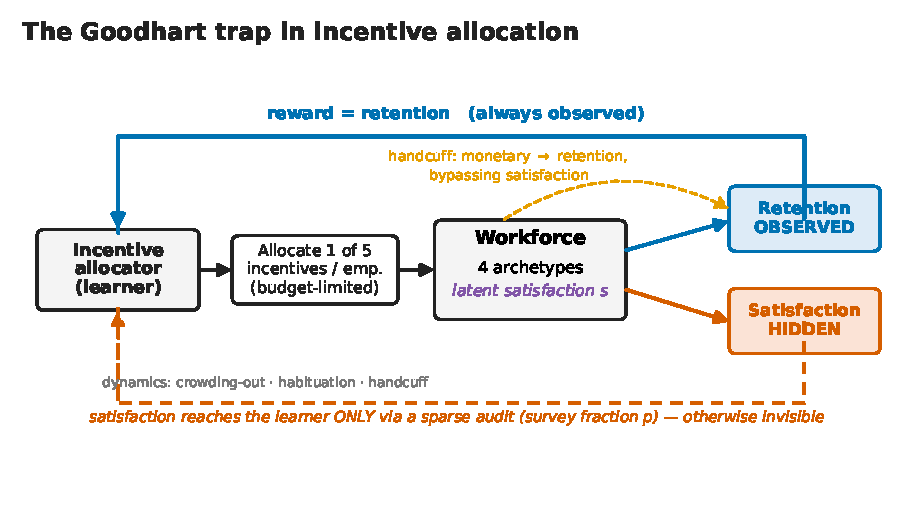
\includegraphics[width=\linewidth]{fig1_schematic.pdf}
  \caption{\emph{(AI-generated schematic.)} The partial-observability incentive
  loop. The allocator's reward sees only \textcolor{blue}{retention}; latent
  \textcolor{red}{satisfaction} returns only through a sparse audit of fraction
  $p$. The \textcolor{orange}{handcuff} channel lets monetary incentives raise
  retention without raising satisfaction, decoupling the optimized proxy from the
  true objective.}
  \label{fig:schematic}
\end{figure}

% =====================================================================
\section{Experimental Setup}
We run every policy for $200$ random seeds at each handcuff strength
$h\in\{0,0.5,1,1.5\}$; the audited learner additionally sweeps
$p\in\{0,0.05,0.1,0.2,0.4\}$ and the three estimators. We report, per run,
\emph{observed retention} per quarter, \emph{mean latent satisfaction}
(unobserved by the allocator), the \emph{archetype gap} (max$-$min mean
satisfaction across archetypes; an equity measure), and, for the confound
controls, mean satisfaction over the never-replaced \emph{founder cohort}.

\textbf{Statistics.} Policy contrasts are paired by seed. We report absolute
mean differences with $95\%$ confidence intervals and, for every directional
claim, the per-seed \emph{sign-stability} (fraction of seeds agreeing on the
sign). We deliberately do \emph{not} headline standardized effect sizes: in a
seed-controlled simulation they measure within-model separation and inflate with
population size, not behavioral magnitude. Kill-test families are corrected with
Benjamini--Hochberg FDR.

\textbf{Validation.} A pre-run battery confirms the learner recovers each
archetype's optimal category under an aligned reward, the attrition hazard is
monotone in $s$, the budget constraint is never violated, and runs are
deterministic per seed.

\textbf{Pre-registered kill-tests.} Before the confirmatory runs we registered
four falsification conditions, each targeting a way the headline could be an
artifact: (K1) if the satisfaction gap vanishes at zero crowding-out, it is
merely a set constant; (K2) if it vanishes on the founder cohort, it is
survivorship composition; (K3) if the audit backfire vanishes under a
precision-aware estimator, it is an estimator artifact; (K4) if signs flip
across a randomized parameter sweep, the findings are not robust.

% =====================================================================
\section{Results}\label{sec:results}
\textbf{The learner degrades the objective it cannot see while matching the
baseline on the one it can.} At the main configuration ($h{=}1$,
Table~\ref{tab:main}, Fig.~\ref{fig:goodhart}), the Learner and the Static
baseline are statistically indistinguishable on observed retention
($0.941$ vs.\ $0.941$; paired difference $-0.0005$, sign-stability $54\%$), yet
the Learner's latent satisfaction is far below ($0.529$ vs.\ $0.566$; paired
difference $-0.037$ $[95\%\,\text{CI}\;\pm0.002]$, $100\%$ sign-stable) and its
archetype inequality is roughly tripled ($0.066$ vs.\ $0.021$). The gap on the
observed metric even reverses sign with the handcuff channel: the Learner is
\emph{worse} than Static on retention at $h{=}0$ ($+0.0061$), tied at $h{=}1$,
and \emph{better} at $h{=}1.5$ ($-0.0059$)---it ``wins'' on the observable proxy
precisely where that proxy is most decoupled from welfare.

\textbf{The degradation is genuine harm, not survivorship composition, and not a
hand-set constant.} We registered two ways this headline could be an artifact
and tested both (Fig.~\ref{fig:decomp}). At \emph{zero} crowding-out and
\emph{zero} handcuff---every welfare-suppressing channel switched off---the
Static$-$Learner satisfaction gap does not vanish but remains
$+0.0151\,[\pm0.0010]$ ($98\%$ sign-stable), attributable to the learner's
exploration cost and habituation; crowding-out and the handcuff then amplify it
monotonically. Restricting the metric to the never-left \emph{founder} cohort
leaves the gap essentially unchanged ($+0.0141\,[\pm0.0011]$), so it is
per-person harm rather than the retention of already-unhappy workers; the gap is
likewise robust to not replacing leavers ($+0.024$) and to drawing replacements
from the survivor distribution ($+0.049$). K1 and K2 do not fire. We therefore
read RQ1/RQ2 as a heterogeneous-agent instantiation of multitask agency
\citep{holmstrom1991}: a robust, decomposed, but theoretically anticipated
effect.

\begin{table}[t]
  \centering
  \caption{Main configuration ($h{=}1$, $200$ seeds, $\pm$ = $95\%$ CI). Higher
  retention and satisfaction are better; lower archetype gap is more equitable.
  The Learner matches Static on the observed metric while degrading the two
  unobserved ones. Regenerates from \texttt{results/full.csv}.}
  \label{tab:main}
  \small
  \begin{tabular}{lcccc}
    \toprule
    Policy & Retention/qtr & Latent satisf. & Archetype gap & Monetary share \\
    \midrule
    Random              & $0.938$ & $0.541$ & $0.034$ & 0.16 \\
    Monetary-only       & $0.944$ & $0.467$ & $0.154$ & 0.50 \\
    Static (theory)     & $0.941$ & $\mathbf{0.566}$ & $\mathbf{0.021}$ & 0.19 \\
    Learner (retention) & $0.941$ & $0.529$ & $0.066$ & 0.25 \\
    Learner + audit ($p{=}.1$) & $0.942$ & $0.525$ & $0.082$ & 0.28 \\
    Oracle (true $s$)   & $0.943$ & $0.542$ & $0.069$ & 0.25 \\
    \bottomrule
  \end{tabular}
\end{table}

\begin{figure}[t]
  \centering
  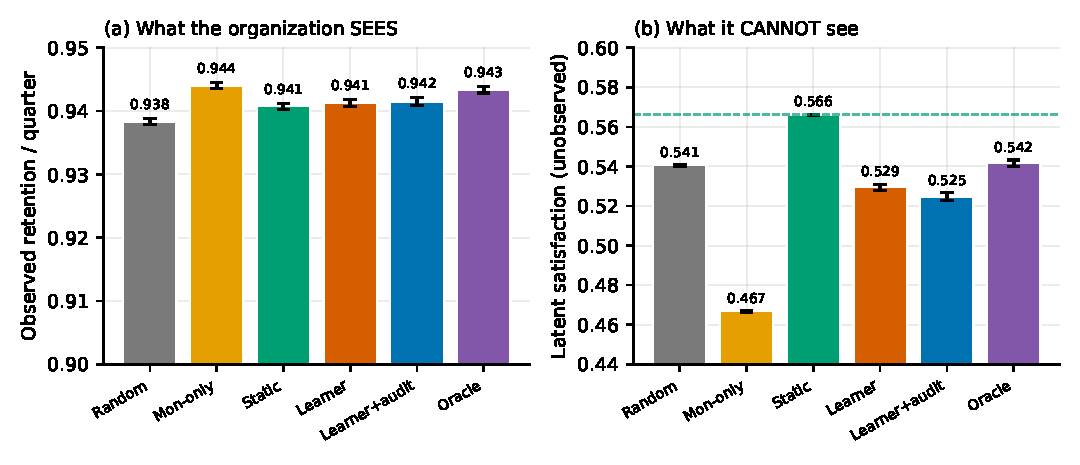
\includegraphics[width=\linewidth]{fig2_goodhart.pdf}
  \caption{\emph{(AI-generated.)} $h{=}1$, $200$ seeds, $95\%$ CI. \textbf{(a)}
  What the organization observes (retention): the Learner matches Static.
  \textbf{(b)} What it cannot see (latent satisfaction): the Learner falls well
  below Static (dashed line). The two panels use the same policies; only the
  measured axis differs.}
  \label{fig:goodhart}
\end{figure}

\begin{figure}[t]
  \centering
  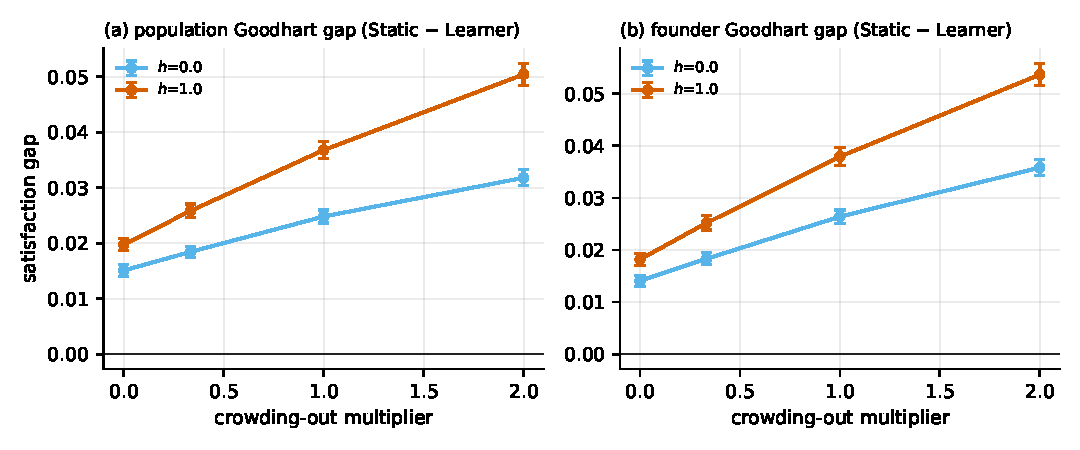
\includegraphics[width=\linewidth]{fig6_decomposition.pdf}
  \caption{\emph{(AI-generated.)} Static$-$Learner satisfaction gap vs.\ the
  crowding-out multiplier, for the full population (a) and the never-left founder
  cohort (b). The gap is nonzero with all amplifiers off (crowding $=0$, and
  $h{=}0$, left points), then grows with crowding and with the handcuff $h$. The
  founder panel rules out survivorship composition. $200$ seeds, $95\%$ CI.}
  \label{fig:decomp}
\end{figure}

\textbf{The welfare and equity erosion survives calibration to a real benchmark.}
To test whether the effect is an artifact of illustrative parameters, we
calibrated the two most load-bearing choices to the IBM HR Analytics benchmark
($n{=}1470$; Fig.~\ref{fig:calib}): the satisfaction$\to$attrition hazard slope,
by logistic regression of attrition on job satisfaction, and the archetype mix,
by clustering. The fitted slope is $0.75$--$0.95$ (vs.\ our illustrative $3.2$),
the archetype mix is skewed (low-compensation $39\%$ vs.\ an equal-share $25\%$),
and---notably---an off-satisfaction retention channel is empirically present: a
stock-option coefficient of $-0.51$ $[-0.72,-0.31]$ controlling for satisfaction,
grounding the ``handcuff'' construct in data. Re-running with the fitted slope and
real mix, the welfare gap holds ($+0.033$ vs.\ $+0.037$ illustrative) and the
equity gap is if anything larger ($+0.047$ vs.\ $+0.045$); both persist on the
founder cohort. The distributional erosion is thus not a parameter artifact.

\textbf{The audit remedy: an honest negative result.} The natural remedy is to
survey a fraction $p$ of employees and reward the learner on measured
satisfaction. We initially observed, with a naive \texttt{raw} estimator, a
striking backfire---auditing at $p{=}0.05$ yielding \emph{lower} satisfaction
than no audit ($-0.0085$, $p_{\text{FDR}}{<}10^{-13}$ at $h{=}0$)---as a
low-precision estimate enters the argmax at full weight and flips allocations on
noise. Two pre-registered tests dismantle the strong version of this claim
(Fig.~\ref{fig:estimator}). First (K3), a precision-weighted \texttt{shrink}
estimator removes the backfire entirely (non-significant after FDR at both $h$).
Second, and more decisively, under the \emph{calibrated} (weaker) hazard slope
the backfire vanishes even for the \texttt{raw} estimator ($+0.003$): it required
a strong satisfaction--retention coupling the benchmark does not exhibit. We
therefore report a negative result: naive auditing backfires only in a narrow
regime (strong coupling $\times$ naive estimator); under realistic coupling or
competent estimation, auditing the hidden objective is roughly neutral-to-helpful.
Audit design and the coupling regime, not audit frequency, determine whether
measurement helps---and in the calibrated regime the remedy neither hurts nor
much helps.

\begin{figure}[t]
  \centering
  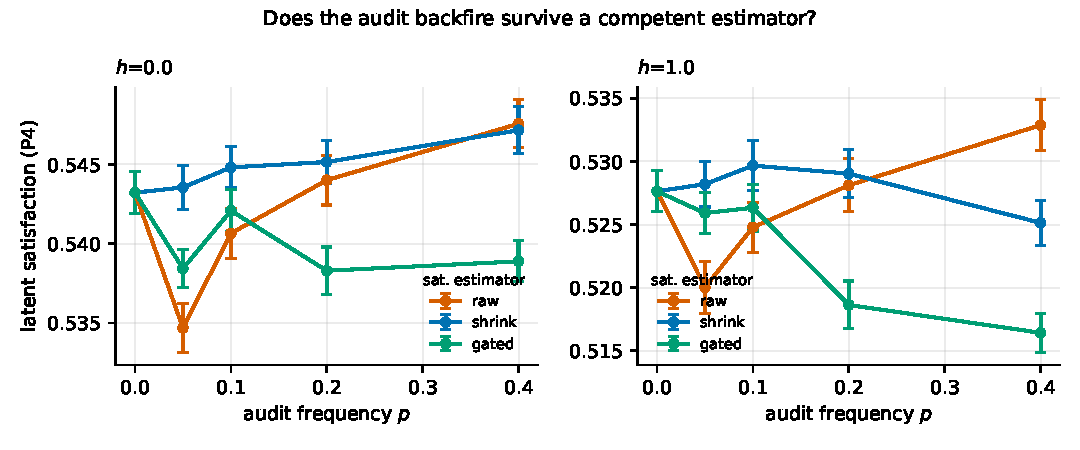
\includegraphics[width=\linewidth]{fig7_estimator.pdf}
  \caption{\emph{(AI-generated.)} The audit backfire is an estimator artifact.
  Audited-learner satisfaction vs.\ audit frequency $p$ under a naive
  running-mean (\texttt{raw}), a precision-weighted (\texttt{shrink}), and a
  confidence-gated (\texttt{gated}) satisfaction estimator. The low-$p$ dip under
  \texttt{raw} is removed by \texttt{shrink} (non-significant after FDR at both
  $h$). $200$ seeds, $95\%$ CI.}
  \label{fig:estimator}
\end{figure}

\begin{figure}[t]
  \centering
  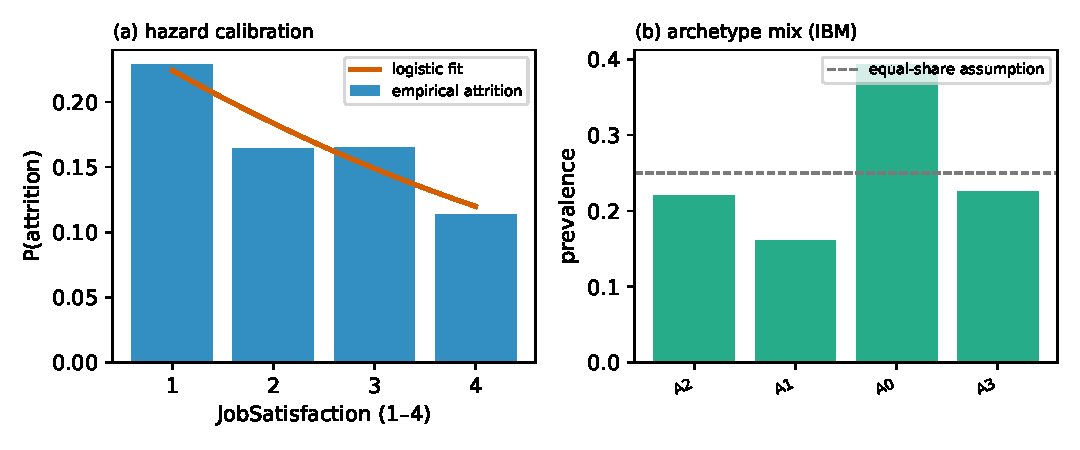
\includegraphics[width=\linewidth]{fig10_calibration.pdf}
  \caption{\emph{(AI-generated.)} Calibration to the IBM HR Analytics benchmark
  ($n{=}1470$). \textbf{(a)} Empirical attrition falls monotonically with job
  satisfaction; logistic fit overlaid (slope $0.75$--$0.95$, vs.\ our illustrative
  $3.2$). \textbf{(b)} The archetype mix departs from the equal-share assumption
  (dashed): low-compensation employees are $39\%$ of the workforce. The
  welfare/equity erosion holds under these fitted values.}
  \label{fig:calib}
\end{figure}

\textbf{Robustness.} Over $250$ randomized worlds (gains, crowding, and hazard
slope drawn over plausible ranges) the population and founder welfare-gap signs
and the equity-gap sign hold in $100\%$ of worlds, while the raw audit backfire
holds in only $62\%$ (Appendix Fig.~\ref{fig:robust})---quantifying which claims
are robust (the welfare/equity erosion) and which are regime-specific (the naive
backfire).

% =====================================================================
\section{Discussion}
Two implications follow. First, and robustly (across randomized worlds and under
benchmark calibration), an allocator evaluated only on the metric it optimizes
can look healthy while eroding an unmeasured objective and---more sharply---its
\emph{fair distribution} across worker types, looking \emph{healthiest} exactly
where the proxy is most decoupled from welfare. The distributional consequence,
not just the average, is what an aggregate KPI hides. Second, and more soberly:
the intuitive fix of occasionally measuring the true objective is, under
realistic (benchmark-calibrated) conditions, roughly neutral---it neither
reliably helps nor, once estimated with basic care, hurts. The naive-auditing
backfire we first found was a fragile, strong-coupling phenomenon, not a general
law; we report it as such. The actionable message is therefore about
\emph{measurement of distribution}, not a silver-bullet audit remedy: track
per-cohort welfare, because the aggregate will not show you where the harm lands.

% =====================================================================
\section{Limitations}
\textbf{Simulation realism.} The study is a conditional model. We calibrate the
two most load-bearing quantities (the satisfaction$\to$attrition hazard slope and
the archetype mix) to the IBM HR Analytics benchmark, but the benchmark is itself
a synthetic dataset and its satisfaction is a cross-sectional self-report, so the
satisfaction \emph{dynamics} (gains, crowding, habituation) remain illustrative;
magnitudes are structural, not field-estimated. The defense against ``you assumed
your conclusion'' is the joint evidence of the randomized-world sweep, the
zero-crowding control, and the benchmark calibration---not any single parameter.
\textbf{Response-model family.} A single functional family is used for the
dynamics; a follow-up should calibrate these to a longitudinal
turnover-and-engagement panel, which our cross-sectional benchmark cannot supply.
\textbf{Learner class.} The optimizer is a
cohort $\varepsilon$-greedy bandit; a contextual learner might shift magnitudes,
though a stronger optimizer on the same misaligned proxy should, if anything,
degrade welfare more. \textbf{Welfare accounting.} We do not track post-exit
outside options; ``degradation'' is a within-model latent, not a claim about
lifetime worker welfare.

% =====================================================================
\section{Conclusion}
Optimizing an observable retention proxy degrades unobserved satisfaction and,
more sharply, its fair distribution across worker types---an effect that survives
a zero-crowding control, a founder-cohort test, a $250$-world randomized sweep,
and calibration of the hazard slope and archetype mix to a real HR benchmark, in
which the off-satisfaction retention channel is itself empirically present. We
frame this as a distributional sharpening of multitask agency rather than a new
mechanism: the contribution is the calibrated, falsification-tested demonstration
and the equity axis, not the aggregate Goodhart effect, which is anticipated. The
intuitive remedy---auditing the hidden objective---we report honestly as a
near-null under realistic conditions: the naive-auditing backfire we first found
was a fragile, strong-coupling phenomenon that vanishes under competent estimation
or benchmark-calibrated coupling. The durable lesson is to measure the
\emph{distribution} of the true objective, not merely its average, because an
aggregate proxy hides where the harm concentrates. We release the testbed, the
pre-registered kill-tests, and the calibration so these findings can be pushed
further toward field data.

\begin{figure}[t]
  \centering
  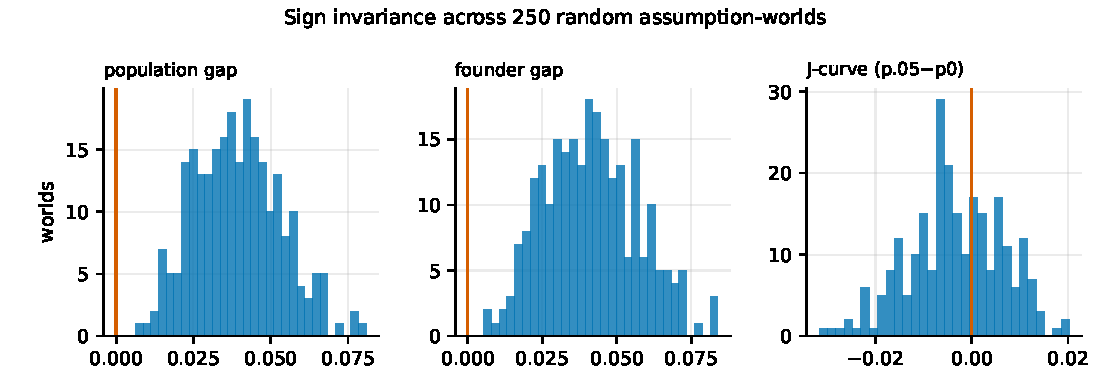
\includegraphics[width=0.92\linewidth]{fig9_robust.pdf}
  \caption{\emph{(AI-generated.)} Sign invariance across $250$ randomized
  assumption-worlds. Population and founder Goodhart-gap signs hold in $100\%$ of
  worlds (mass entirely $>0$); the raw-estimator audit backfire holds in $62\%$
  (mass straddles $0$)---quantifying which findings are robust and which are not.}
  \label{fig:robust}
\end{figure}

% =====================================================================
\section*{Acknowledgments and disclosure}
Simulation code, analysis code, and figure rendering were AI-assisted (a large
language model). The research questions, experimental-design decisions, execution
of the experiments of record, interpretation, and the intellectual content are
the author's own; an AI-use prompt log is available on request. Adversarial review of an earlier
draft (which surfaced the estimator-artifact hypothesis subsequently confirmed
by kill-test K3) was AI-assisted and is likewise logged.

% =====================================================================
% References: verified real (canonical details checked); confirm each against
% the original before submission and assemble the
% bibliography independently.
\begin{thebibliography}{99}
\small
\bibitem{amodei2016} Amodei, D., Olah, C., Steinhardt, J., Christiano, P., Schulman, J., \& Man\'e, D. (2016). Concrete Problems in AI Safety. \emph{arXiv:1606.06565}.
\bibitem{baker1992} Baker, G.\ (1992). Incentive Contracts and Performance Measurement. \emph{Journal of Political Economy}, 100(3), 598--614.
\bibitem{cheng2020} Cheng, X.\ (2020). Obtain Employee Turnover Rate and Optimal Reduction Strategy Based on Neural Network and Reinforcement Learning. \emph{arXiv:2012.00583}.
\bibitem{deci1999} Deci, E.\ L., Koestner, R., \& Ryan, R.\ M.\ (1999). A meta-analytic review of experiments examining the effects of extrinsic rewards on intrinsic motivation. \emph{Psychological Bulletin}, 125(6), 627--668.
\bibitem{dickinson2008} Dickinson, D., \& Villeval, M.-C.\ (2008). Does monitoring decrease work effort? The complementarity between agency and crowding-out theories. \emph{Games and Economic Behavior}, 63(1), 56--76.
\bibitem{falk2006} Falk, A., \& Kosfeld, M.\ (2006). The Hidden Costs of Control. \emph{American Economic Review}, 96(5), 1611--1630.
\bibitem{frey2001} Frey, B.\ S., \& Jegen, R.\ (2001). Motivation Crowding Theory. \emph{Journal of Economic Surveys}, 15(5), 589--611.
\bibitem{gao2023} Gao, L., Schulman, J., \& Hilton, J.\ (2023). Scaling Laws for Reward Model Overoptimization. \emph{ICML} (PMLR 202).
\bibitem{herzberg1959} Herzberg, F., Mausner, B., \& Snyderman, B.\ B.\ (1959). \emph{The Motivation to Work}. Wiley. [Two-factor theory; note it is contested in modern I/O psychology, e.g.\ House \& Wigdor 1967.]
\bibitem{holmstrom1991} Holmstr\"om, B., \& Milgrom, P.\ (1991). Multitask Principal-Agent Analyses: Incentive Contracts, Asset Ownership, and Job Design. \emph{Journal of Law, Economics, \& Organization}, 7(Special Issue), 24--52.
\bibitem{karwowski2024} Karwowski, J., et al.\ (2024). Goodhart's Law in Reinforcement Learning. \emph{ICLR}. arXiv:2310.09144.
\bibitem{krakovna2020} Krakovna, V., et al.\ (2020). Specification gaming: the flip side of AI ingenuity. \emph{DeepMind Blog}.
\bibitem{ryandeci2000} Ryan, R.\ M., \& Deci, E.\ L.\ (2000). Self-determination theory and the facilitation of intrinsic motivation, social development, and well-being. \emph{American Psychologist}, 55(1), 68--78.
\bibitem{skalse2022} Skalse, J., Howe, N.\ H.\ R., Krasheninnikov, D., \& Krueger, D.\ (2022). Defining and Characterizing Reward Hacking. \emph{NeurIPS}. arXiv:2209.13085.
\bibitem{strathern1997} Strathern, M.\ (1997). `Improving ratings': audit in the British University system. \emph{European Review}, 5(3), 305--321.
\end{thebibliography}

\end{document}
